% !TEX TS-program = pdflatex
% !TEX encoding = UTF-8 Unicode
\documentclass[fleqn,12pt, a4paper]{article}
% Русский язык
\usepackage[T2A, T1]{fontenc}
\usepackage[utf8]{inputenc}
\usepackage[english,russian]{babel}

 % Поля страницы
\usepackage{geometry}
\geometry{left=2cm}
\geometry{right=1.5cm}
\geometry{top=2cm}
\geometry{bottom=2cm}

\usepackage[pdftex]{graphicx}
\graphicspath{{images/}}%путь к рисункам
\DeclareGraphicsExtensions{.png}

\usepackage{pgf}
\usepackage{tikz}
\usetikzlibrary{arrows,automata,positioning}
\usetikzlibrary{shapes.misc}

%\usepackage{indentfirst} % включить отступ у первого абзаца

\usepackage{booktabs} % for much better looking tables
\usepackage{array} % for better arrays (eg matrices) in maths
\usepackage{multirow}
\usepackage{paralist} % very flexible & customisable lists (eg. enumerate/itemize, etc.)
\usepackage{enumitem }
%\usepackage{amsmath}
\usepackage[fleqn]{amsmath}
\setlength{\mathindent}{0pt}
\usepackage{amsfonts,amssymb,amsthm,epsfig,epstopdf,titling,url,array,nccmath }

\usepackage{listings} % for source code highlighning
\lstset{language=C++}

% Переопределения
\newcommand {\la} {\langle}
\newcommand {\ra} {\rangle}
\renewcommand {\le} {\leqslant}
\renewcommand {\ge} {\geqslant}
\renewcommand {\leq} {\leqslant}
\renewcommand {\geq} {\geqslant}
\renewcommand {\emptyset} {\varnothing}
\newcommand {\es} {\varnothing}
\newcommand {\eps} {\varepsilon}
\newcommand {\mydef}[1]{\emph{#1}}
\newcommand{\To}{\Rightarrow}

\newcommand{\Sig}{\ensuremath{\Sigma}}
\newcommand{\N}{\ensuremath{\mathbb N}}
\newcommand{\NO}{\ensuremath{\mathbb N_0}}

% Неразрывный дефис, который допускает перенос внутри слов,
% типа жёлто-синий: нужно писать жёлто"/синий.
\makeatletter
    \defineshorthand[russian]{"/}{\mbox{-}\bbl@allowhyphens}
\makeatother
% Конец переопределений

\begin{document}

%%%%%%%%%%%%%%%%%%%%%%%%%%%%%%%%%%%%%%%
%						Титульный лист						%
%%%%%%%%%%%%%%%%%%%%%%%%%%%%%%%%%%%%%%%

\begin{titlepage}

\begin{center}
\MakeUppercase{Минобрнауки России}\\
Федеральное государственное автономное образовательное учреждение
высшего профессионального образования
<<Южный федеральный университет>>\\[1 cm]

Институт математики, механики и компьютерных наук им. И.И. Воровича\\[1 cm]

Кафедра алгебры и дискретной математики\\[5cm]

\Huge \MakeUppercase{Курсовая работа} \\[0.6cm]

\large по предмету: <<Теория автоматов и формальных языков>>\\[7cm]

\end{center}

\begin{flushleft}
{\large
Выполнил: \\
Студент 3 курса, 9 группы \hfill Стребежев Игорь \\[1cm]

Проверил:\\
к.т.н., ст. преп. кафедры АДМ \hfill Е.В. Алымова}

\end{flushleft}
\vfill

\begin{center}
Ростов-на-Дону\\
\the\year
\end{center}
\end{titlepage}

%%%%%%%%%%%%%%%%%%%%%%%%%%%%%%%%%%%%%%%
%		Текст курсовой
%%%%%%%%%%%%%%%%%%%%%%%%%%%%%%%%%%%%%%%

\section*{Задание 1}

Вариант 18. Язык над алфавитом $\Sigma = \{ 0, 1 \} $, состоящий из всех слов, в которых после третьей слева единицы стоит четное число групп вида 01.

\begin{enumerate}[label=(\roman{*})]
	\item Построить ПЛ-грамматику $G$, порождающую $L$.

	\begin{equation}
		\begin{array}{l}
			S \to 0S \mid 1A, \\
			A \to 0A \mid 1B, \\
			B \to 0B \mid 1C \mid 1, \\
			C \to 0101C \mid 0101;
		\end{array}
	\end{equation}

	\item Доказать вложения $L \subseteq L(G)$, $L(G) \subseteq L$.\\

	\underline{$L \subseteq L(G)$}: Рассмотрим дерево выводов грамматики.

	$S \implies 0S \implies 00S \implies 000S \implies \dots$ --- нули разрешены в начале слов в $L$.

	$S \implies 1A \implies 10A \implies 100A \implies \dots$ --- генерация первой единицы и последовательности нулей.

	Первые три правила грамматики одинаковы и образуют три пары из последовательности (возможно пустой) нулей и единицы. Что также удовлетворяет описанию языка~$L$.

	$11B \implies 111 $ --- в таком случае количество групп вида 01 будет равно нулю (чётно), принадлежит языку.

	$11B \implies 111C \implies 111\ 0101$ --- генерация пары групп.

	$11B \implies 111C \implies 111\ 0101C \implies 111\ 0101\ 0101$ --- всегда чётное количество групп.

	Таким образом все слова, порождаемые грамматикой $G$ принадлежат языку $L$, то есть $L \subseteq L(G)$.\\


	\underline{$L(G) \subseteq L$}: Язык L имеет структуру $(0^*1)(0^*1)(0^*1)(1010)^*$, каждая цепочка этого языка описывает все терминальные выводы из правил
	 грамматики, как показано в предыдущем пункте, что и доказывает вложение.

	\item Путём решения системы линейных уравнений с регулярными коэффициентами построить регулярное выражение, описывающее $L$.


	\begin{equation}
		\begin{array}{l}
		S = 0S + 1A, \\
		A = 0A + 1B, \\
		B = 0B + 1C + 1, \\
		C = 0101C + 0101; \\\\

		C = (0101)^*0101 = 0101^+, \\
		B = 0B + 1(0101^+ + \eps) = 0^* 1(0101^+ + \eps), \\
		A = 0A + 1(0^* 1(0101^+ + \eps)) = 0^* 1(0^* 1(0101^+ + \eps)), \\
		S = 0S + 1(0^* 1(0^* 1(0101^+ + \eps))) = 0^* 1(0^* 1(0^* 1(0101^+ + \eps))); \\\\

		0^* 1(0^* 1(0^* 1(0101^+ + \eps))) = (0^*1) (0^*1) (0^*1) (0101)^*.
		\end{array}
	\end{equation}


	\item Построить НКА или \emph{e}-НКА $M^{ND}$, распознающий язык $L$, предъявить его граф. \\

	\begin{tikzpicture}[auto,>=stealth', node distance=3cm,auto,every state/.style={thick}]
		\node (init) {};
		\node[state] (qS) [right=.7cm of init] {$S$};
		\node[state] (qA) [right of=qS] {$A$};
		\node[state] (qB) [right of=qA] {$B$};
		\node[state] (qC) [right of=qB] {$C$};
		\node[state,accepting] (qF) [below of=qB] {$F$};
		\node[state,accepting] (qE) [below of=qC] {$E$};

		\path[->]
		(init) edge (qS)
		(qS) edge [loop above] node {$0$} (qS)
		(qS) edge node {$1$} (qA)
		(qA) edge [loop above] node {$0$} (qA)
		(qA) edge node {$1$} (qB)
		(qB) edge [loop above] node {$0$} (qB)
		(qB) edge node {$1$} (qF)
		(qB) edge node {$1$} (qC)
		(qC) edge [loop above] node {$0101$} (qC)
		(qC) edge node {$0101$} (qE)
		;
	\end{tikzpicture}

	\item Построить ДКА $M^D$ путём детерминизации $M^{ND}$, предъявить его граф. \\

	Построим таблицу переходов $M^{ND}$.

	\begin{tabular}{lcccccccccccc}
		\toprule
		\multicolumn{1}{c}{
			$\delta^\prime \mid$
		}
		& \multicolumn{1}{c}{ $S$ }
		& \multicolumn{1}{c}{ $A$ }
		& \multicolumn{1}{c}{ $B$ }
		& \multicolumn{1}{c}{ $C$ }
		& \multicolumn{1}{c}{ $K^0$ }
		& \multicolumn{1}{c}{ $K^{01}$ }
		& \multicolumn{1}{c}{ $K^{010}$ }
		& \multicolumn{1}{c}{ $E^0$ }
		& \multicolumn{1}{c}{ $E^{01}$ }
		& \multicolumn{1}{c}{ $E^{010}$ }
		& \multicolumn{1}{c}{ $E$ }
		& \multicolumn{1}{c}{ $F$ }
		\\
		\midrule

		0 $\mid$ &
		$S$ & $A$ & $B$ & $\{K^0, E^0\}$ & --- & $K^{010}$ & --- & --- & $E^{010}$ & --- & --- & --- \\
		1 $\mid$ &
		$A$ & $B$ & $\{ C, F \}$ & --- & $K^{01}$ & --- & $C$ & $E^{01}$ & --- & $E$ & --- & ---	\\
		\bottomrule
	\end{tabular}

	\vspace{1em}

	Расширим таблицу при приведении автомата в $M^D$.


	\begin{tabular}{lcccccccc}
		\toprule
		\multicolumn{1}{c}{
			$\delta^\prime \mid$
		}
		& \multicolumn{1}{c}{ $S$ }
		& \multicolumn{1}{c}{ $A$ }
		& \multicolumn{1}{c}{ $B$ }
		& \multicolumn{1}{c}{ $\{C, F\}$ }
		& \multicolumn{1}{c}{ $\{K^{ 0 }, E^{ 0 }\}$ }
		& \multicolumn{1}{c}{ $\{K^{ 01 }, E^{ 01 }\}$ }
		& \multicolumn{1}{c}{ $\{K^{ 010 }, E^{ 010 }\}$ }
		& \multicolumn{1}{c}{ $\{ C, E \}$ }
		\\
		\midrule

		0 $\mid$ &
		$S$ & $A$ & $B$ &  $\{K^0, E^0\}$ & --- & $\{K^{ 010 }, E^{ 010 }\}$ & --- &  $\{K^{ 0 }, E^{ 0 }\}$  \\
		1 $\mid$ &
		$A$ & $B$ & $\{ C, F \}$ & --- &  $\{K^{ 01 }, E^{ 01 }\}$ & --- & $\{ C, E \}$ & ---	\\
		\bottomrule
	\end{tabular}

	\vspace{1em} Отобразим этот автомат на диаграмме.


	\begin{tikzpicture}[auto,>=stealth', node distance=3cm,auto,every state/.style={thick}]
		\node (init) {};
		\node[state] (qS) [right=.7cm of init] {$S$};
		\node[state] (qA) [right of=qS] {$A$};
		\node[state] (qB) [right of=qA] {$B$};
		\node[state,accepting] (qCF) [right of=qB] {$CF$};
		\node[state] (qKE) [right of=qCF] {$K^0E^0$};
		\node[state,accepting] (qCE) [right of=qKE] {$CE$};

		\path[->]
		(init) edge (qS)
		(qS) edge [loop above] node {$0$} (qS)
		(qS) edge node {$1$} (qA)
		(qA) edge [loop above] node {$0$} (qA)
		(qA) edge node {$1$} (qB)
		(qB) edge [loop above] node {$0$} (qB)
		(qB) edge node {$1$} (qCF)
		(qCF) edge node {$0$} (qKE)

		(qKE) edge  [bend left] node {$101$} (qCE)
		(qCE) edge  [bend left] node {$0$} (qKE)
		;
	\end{tikzpicture}
\end{enumerate}

\newpage
\section*{Задание 2}
Вариант 29. $\Sigma = \{ 0, 1, 2, 3, 4, 5 \}$, $A = \{ 53150, 53555, 5510, 0001 \}$.

\begin{enumerate}
	\item Для каждого слова $w_i \in A$ построить НКА $M_i^{ND}$, распознающий наличие в произвольной строке $s \in \Sigma^*$ подстроки $w_i$.
	\item Для каждого НКА $M_i^{ND}$ построить соответствующий ДКА $M_i^{D}$.\\

	Слово 53150.\\

	\begin{tikzpicture}[auto,>=stealth', node distance=3cm,auto,every state/.style={thick}]
		\node (init) {};
		\node[state] (S) [right=.7cm of init] {$S$};
		\node[state] (qA1) [below of=qS] {$A^1$};
		\node[state] (qA2) [right of=qA1] {$A^2$};
		\node[state] (qA3) [right of=qA2] {$A^3$};
		\node[state] (qA4) [right of=qA3] {$A^4$};
		\node[state] (qA5) [right of=qA4] {$A^5$};
		\node[state,accepting] (qA6) [right of=qA5] {$A^6$};

		\path[->]
		(init) edge (qS)
		(qS) edge [loop above] node {$ 0, 1, 2, 3, 4, 5 $} (qS)
		(qS) edge node {$\eps$} (qA1)
		(qA1) edge node {$5$} (qA2)
		(qA2) edge node {$3$} (qA3)
		(qA3) edge node {$1$} (qA4)
		(qA4) edge node {$5$} (qA5)
		(qA5) edge node {$0$} (qA6)
		(qA6) edge [bend right] node {$\eps$} (qS)
		;
	\end{tikzpicture}

	\vspace{2em}

	\begin{tikzpicture}[auto,>=stealth', node distance=3cm,auto,every state/.style={thick}]
	\node (init) {};
	\node[state] (S) [right=.7cm of init] {$S$};
	\node[state] (q1) [right=3cm of qS] {$A^1$};
	\node[state] (q2) [below of=q1] {$A^2$};
	\node[state] (q3) [below of=q2] {$A^3$};
	\node[state] (q4) [below of=q3, right=0.7cm of q3] {$A^4$};
	\node[state,accepting] (q5) [below right of=q4] {$A^5$};

	\path[->]
	(init) edge (qS)
	(qS) edge [loop above] node {\small{$ 0, 1, 2, 3, 4 $}} (qS)

	(qS) edge [bend left] node {$ 5 $} (q1)
	(q1) edge [bend left] node {\small{$ 0, 1, 2, 3, 4 $}} (qS)

	(q1) edge [loop above] node {$ 5 $} (q1)
	(q1) edge [bend left] node {$3$} (q2)

	(q2) edge [bend left] node {$5$} (q1)
	(q2) edge [bend left=10] node {\small{$0, 2, 3, 4$}} (qS)
	(q2) edge node {$1$} (q3)

	(q3) edge node {$5$} (q4)
	(q3) edge [bend left] node[right] {\small{$0, 1, 2, 3, 4$}} (qS)

	(q4) edge [bend right] node {$3$} (q2)
	(q4) edge [bend right] node {$5$} (q1)
	(q4) edge [bend left=40] node {\small{$1, 2, 4$}} (qS)

	(q4) edge node {$0$} (q5)

	(q5) edge [bend right] node {$5$} (q1)
	(q5) edge [bend left=60] node {\small{$0, 1, 2, 3, 4$}} (qS)
	;
	\end{tikzpicture}

	\newpage
	Слово 53555.\\

	\begin{tikzpicture}[auto,>=stealth', node distance=3cm,auto,every state/.style={thick}]
		\node (init) {};
		\node[state] (S) [right=.7cm of init] {$S$};
		\node[state] (qA1) [below of=qS] {$B^1$};
		\node[state] (qA2) [right of=qA1] {$B^2$};
		\node[state] (qA3) [right of=qA2] {$B^3$};
		\node[state] (qA4) [right of=qA3] {$B^4$};
		\node[state] (qA5) [right of=qA4] {$B^5$};
		\node[state,accepting] (qA6) [right of=qA5] {$B^6$};

		\path[->]
		(init) edge (qS)
		(qS) edge [loop above] node {$ 0, 1, 2, 3, 4, 5 $} (qS)
		(qS) edge node {$\eps$} (qA1)
		(qA1) edge node {$5$} (qA2)
		(qA2) edge node {$3$} (qA3)
		(qA3) edge node {$5$} (qA4)
		(qA4) edge node {$5$} (qA5)
		(qA5) edge node {$5$} (qA6)
		(qA6) edge [bend right] node {$\eps$} (qS)
		;
	\end{tikzpicture}

	\vspace{2em}

	\begin{tikzpicture}[auto,>=stealth', node distance=3cm,auto,every state/.style={thick}]
		\node (init) {};
		\node[state] (S) [right=.7cm of init] {$S$};
		\node[state] (q1) [above right of=qS] {$B^1$};
		\node[state] (q2) [right of=q1] {$B^2$};
		\node[state] (q3) [below right of=q2] {$B^3$};
		\node[state] (q4) [right of=q3] {$B^4$};
		\node[state,accepting] (q5) [right of=q4] {$B^5$};

		\path[->]
		(init) edge (qS)
		(qS) edge [loop below] node [left] {\small{$ 0, 1, 2, 3, 4 $}} (qS)


		(qS) edge [bend left] node {$ 5 $} (q1)

		(q1) edge [bend left] node [right] {\small{$ 0, 1, 2, 4 $}} (qS)
		(q1) edge [loop above] node {$ 5 $} (q1)
		(q1) edge node {$3$} (q2)

		(q2) edge [bend left] node {$5$} (q3)
		(q2) edge [bend left] node {\small{$0, 1, 2, 3, 4$}} (qS)

		(q3) edge [bend left] node {$3$} (q2)
		(q3) edge [bend left] node {\small{$0, 1, 2, 4$}} (qS)
		(q3) edge node {$5$} (q4)

		(q4) edge [bend right=25] node [above] {$3$} (q2)
		(q4) edge [bend left=40] node {\small{$0, 1, 2, 4$}} (qS)
		(q4) edge node {$5$} (q5)

		(q5) edge [bend right] node [above] {$3$} (q2)
		(q5) edge [bend left=60] node {\small{$0, 1, 2, 4$}} (qS)
		(q5) edge [bend right=60] node [above] {$5$} (q1)
		;
	\end{tikzpicture}

	\newpage
	Слово 5510.\\

	\begin{tikzpicture}[auto,>=stealth', node distance=3cm,auto,every state/.style={thick}]
		\node (init) {};
		\node[state] (qS) [right=.7cm of init] {$S$};
		\node[state] (qA1) [right=1cm of qS] {$C^1$};
		\node[state] (qA2) [right of=qA1] {$C^2$};
		\node[state] (qA3) [right of=qA2] {$C^3$};
		\node[state] (qA4) [right of=qA3] {$C^4$};
		\node[state,accepting] (qA5) [right of=qA4] {$C^5$};

		\path[->]
		(init) edge (qS)
		(qS) edge [loop above] node {$ 0, 1, 2, 3, 4, 5 $} (qS)
		(qS) edge node {$\eps$} (qA1)
		(qA1) edge node {$5$} (qA2)
		(qA2) edge node {$5$} (qA3)
		(qA3) edge node {$1$} (qA4)
		(qA4) edge node {$0$} (qA5)
		(qA5) edge [bend right=40, looseness=0.4] node {$\eps$} (qS)
		;
	\end{tikzpicture}

	\vspace{2em}

	\begin{tikzpicture}[auto,>=stealth', node distance=3cm,auto,every state/.style={thick}]
		\node[state] (qS) {$S$};
		\node[state] (q3) [below of=qS] {$C^3$};
		\node[state] (q2) [right of=q3] {$C^2$};
		\node[state,accepting] (q4) [left of=q3] {$C^4$};
		\node[state] (q1) [below of=q3] {$C^1$};

		\path[->]
		(qS) edge [loop above] node [above] {\small{$ 0, 1, 2, 3, 4 $}} (qS)
		(qS) edge [bend left=80, looseness=2.5] node {$ 5 $} (q1)


		(q1) edge [bend left=80, looseness=2.5] node {\small{$ 0, 1, 2, 3, 4 $}} (qS)
		(q1) edge node [below] {$5$} (q2)

		(q2) edge node [above, rotate=-45] {\small{$0, 2, 3, 4$}} (qS)
		(q2) edge [loop above] node {$ 5 $} (q2)
		(q2) edge node {$1$} (q3)

		(q3) edge node {$5$} (q1)
		(q3) edge node [above, rotate=-90] {\small{$1, 2, 3, 4$}} (qS)
		(q3) edge node {$0$} (q4)

		(q4) edge node [below] {$5$} (q1)
		(q4) edge node [above, rotate=45] {\small{$0, 1, 2, 3, 4$}} (qS)
		;
	\end{tikzpicture}

	Слово 0001.\\

	\begin{tikzpicture}[auto,>=stealth', node distance=3cm,auto,every state/.style={thick}]
		\node (init) {};
		\node[state] (qS) [right=.7cm of init] {$S$};
		\node[state] (qA1) [right=1cm of qS] {$D^1$};
		\node[state] (qA2) [right of=qA1] {$D^2$};
		\node[state] (qA3) [right of=qA2] {$D^3$};
		\node[state] (qA4) [right of=qA3] {$D^4$};
		\node[state,accepting] (qA5) [right of=qA4] {$D^5$};

		\path[->]
		(init) edge (qS)
		(qS) edge [loop above] node {$ 0, 1, 2, 3, 4, 5 $} (qS)
		(qS) edge node {$\eps$} (qA1)
		(qA1) edge node {$0$} (qA2)
		(qA2) edge node {$0$} (qA3)
		(qA3) edge node {$0$} (qA4)
		(qA4) edge node {$1$} (qA5)
		(qA5) edge [bend right=40, looseness=0.4] node {$\eps$} (qS)
		;
	\end{tikzpicture}

	\vspace{3em}


	\begin{tikzpicture}[auto,>=stealth', node distance=3cm,auto,every state/.style={thick}]
	\node (init) {};
	\node[state] (S) [right=.7cm of init] {$S$};
	\node[state] (qA1) [right of=qS] {$D^1$};
	\node[state] (qA2) [right of=qA1] {$D^2$};
	\node[state] (qA3) [right of=qA2] {$D^3$};
	\node[state,accepting] (qA4) [right of=qA3] {$D^4$};

	\path[->]
	(init) edge (qS)
	(qS) edge [loop above] node [left] {$ 1, 2, 3, 4, 5 $} (qS)
	(qS) edge node {$0$} (qA1)
	(qA1) edge node {$0$} (qA2)
	(qA2) edge node {$0$} (qA3)
	(qA3) edge node {$1$} (qA4)
	(qA4) edge [bend right=40] node [above] {$0$} (qA1)
	(qA3) edge [loop above] node {$ 0 $} (qA3)

	(qA1) edge [bend right=40] node [above] {$ 1, 2, 3, 4, 5 $} (qS)
	(qA2) edge [bend left=20] node {$ 1, 2, 3, 4, 5 $} (qS)
	(qA3) edge [bend left] node {$ 2, 3, 4, 5 $} (qS)
	(qA4) edge [bend left=40] node {$ 1, 2, 3, 4, 5 $} (qS)
	;
	\end{tikzpicture}
\end{enumerate}

\newpage
\section*{Задание 3}
$L_1 = b^*bba^*(ab + b)^*$, $L_2 = a^*ba^*ab$.
\begin{enumerate}[label=(\roman{*})]
	\item Вычислить регулярное выражение, определяющее язык $L_1 \cap L_2$.

	Рассмотрим множество слов из $L_2$ таких, что их первая буква равна $a$, \\$M = \{ w \mid w \in L_2, w^0 = a \}$. Очевидно, что $ L_1 \cap M = \emptyset$, так как слова из $L_1$ начинаются с буквы $b$. Уберём это множество из рассмотрения, пусть $L_2' = ba^*ab$, где $L_2' \cup M = L_2$.

	В множестве $L_2'$ все слова начинаются со строки ''$ba$'', а в множестве $L_1$ --- ''$bb$''.\\Из этого следует, что $L_1$ и $L_2'$ не пересекаются, а значит $L_1 \cap L_2 = \emptyset$.\\

	\item Вычислить регулярное выражение, определяющее язык $L_1 \bigtriangleup L_2$.

	Согласно определению симметрической разности имеем:\\
	$ L_1 \bigtriangleup L_2 = (L_1 \cup L_2) \setminus (L_1 \cap L_2) = L_1 \cup L_2 = b^*bba^*(ab + b)^* + a^*ba^*ab $.\\

	\item Определить: совпадают ли языки $L_1$ и $L_2$, является ли $L_1$ дополнением $L_2$.

	Так как $L_1 \cap L_2 = \emptyset$, то $L_1 \neq L_2$.\\\\ Предположим, $L_1$ является дополнением $L_2$. Рассмотрим слово $w = "ba"$. Видно, что \\ $w \not\in L_1,\ w \not\in L_2 \To $ наше предположение неверно.

	\item Построить \emph{e}-НКА, распознающий один из языков $L_1^R$ или $L_2^R$.

	Построим $L_2$:

	\begin{tikzpicture}[auto,>=stealth', node distance=2cm,auto,every state/.style={thick}]
	\node (init) {};
	\node[state] (S) [right=.7cm of init] {$0$};
	\node[state] (q1) [right of=qS] {$1$};
	\node[state] (q2) [right of=q1] {$2$};
	\node[state] (q3) [right of=q2] {$3$};
	\node[state] (q4) [right of=q3] {$4$};
	\node[state,accepting] (q5) [right of=q4] {$5$};

	\path[->]
	(init) edge (qS)
	(qS) edge [bend left] node [above] {$a, \eps$} (q1)
	(q1) edge [bend left] node [below] {$\eps$} (qS)

	(q1) edge node {$b$} (q2)

	(q2) edge [bend left] node [above] {$a, \eps$} (q3)
	(q3) edge [bend left] node [below] {$\eps$} (q2)

	(q3) edge node {$a$} (q4)
	(q4) edge node {$b$} (q5)

	;
	\end{tikzpicture}


	Построим $L_2^R$:

	\begin{tikzpicture}[auto,>=stealth', node distance=2cm,auto,every state/.style={thick}]
	\node (init) {};
	\node[state,accepting] (S) [right=.7cm of init] {$0$};
	\node[state,accepting] (q1) [right of=qS] {$1$};
	\node[state,accepting] (q2) [right of=q1] {$2$};
	\node[state,accepting] (q3) [right of=q2] {$3$};
	\node[state,accepting] (q4) [right of=q3] {$4$};
	\node[state] (q5) [right of=q4] {$5$};

	\node[state,accepting] (n2) [below of=q2] {$6$};
	\node[state,accepting] (n5) [right of=q5] {$8$};

	\path[->]
	(init) edge (qS)
	(qS) edge [bend left] node [above] {$a, \eps$} (q1)
	(q1) edge [bend left] node [below] {$\eps$} (qS)

	(q1) edge node {$b$} (q2)

	(q2) edge [bend left] node [above] {$a, \eps$} (q3)
	(q3) edge [bend left] node [below] {$\eps$} (q2)

	(q3) edge node {$a$} (q4)
	(q4) edge node {$b$} (q5)

	(q2) edge node {$b$} (n2)
	(n2) edge [loop left] node [above] {$a, b$} (n2)

	(q5) edge node {$a, b$} (n5)
	(n5) edge [loop right] node [above] {$a, b$} (n5)

	;
	\end{tikzpicture}

	\item Вычислить регулярное выражение по построенному \emph{e}-НКА.

	Упростим построенный в предыдущем пункте автомат, используя метод исключения.

	\begin{tikzpicture}[auto,>=stealth', node distance=2cm,auto,every state/.style={thick}]
	\node (init) {};
	\node[state,accepting] (qS) [right=.7cm of init] {$0$};
	\node[state,accepting] (q2) [right=3cm of qS] {$2$};
	\node[state,accepting] (q4) [right=3cm of q2] {$4$};

	\node[state,accepting] (n2) [below of=q2] {$6$};
	\node[state,accepting] (n5) [right=2cm of q4] {$8$};

	\path[->]
	(init) edge (qS)
	(qS) edge [loop above] node [left] {$a$} (qS)

	(qS) edge node {$b$} (q2)

	(q2) edge [loop above] node [left] {$a$} (q2)

	(q2) edge node {$a$} (q4)

	(q2) edge node {$b$} (n2)
	(n2) edge [loop left] node [above] {$a, b$} (n2)

	(q4) edge node [above] {$b(a+b)^+$} (n5)

	;
	\end{tikzpicture}

	Опишем заключающее состояние в вершине 8: $R = a^*ba^*ab(a+b)^+$.
	\newpage

	Уберём вершину 8, опишем состояние в вершине 4:
	$R = a^*ba^*a\ (\eps + b(a+b)^+) $.

	\begin{tikzpicture}[auto,>=stealth', node distance=2cm,auto,every state/.style={thick}]
	\node (init) {};
	\node[state,accepting] (qS) [right=.7cm of init] {$0$};
	\node[state,accepting] (q2) [right=3cm of qS] {$2$};
	\node[state,accepting] (q4) [right=3.5cm of q2] {$4$};

	\node[state,accepting] (n2) [below of=q2] {$6$};

	\path[->]
	(init) edge (qS)
	(qS) edge [loop above] node [left] {$a$} (qS)

	(qS) edge node {$b$} (q2)

	(q2) edge [loop above] node [left] {$a$} (q2)

	(q2) edge node {$a\ (\eps + b(a+b)^+)$} (q4)

	(q2) edge node {$b(a+b)^*$} (n2)
	;
	\end{tikzpicture}

	Уберём вершины 4, 6, опишем состояние в вершине 2:\\
	$R = a^*ba^*\ (\eps\ +\ b(a+b)^* +\ a (\eps + b(a+b)^+)) $.

	\vspace{1em}

	\begin{tikzpicture}[auto,>=stealth', node distance=2cm,auto,every state/.style={thick}]
	\node (init) {};
	\node[state,accepting] (qS) [right=.7cm of init] {$0$};
	\node[state,accepting] (q2) [right=3cm of qS] {$2$};

	\path[->]
	(init) edge (qS)
	(qS) edge [loop above] node [left] {$a$} (qS)

	(qS) edge node {$b$} (q2)

	(q2) edge [loop above] node [left] {$a$} (q2)
	;
	\end{tikzpicture}

	\vspace{1em}

	Данный автомат можно описать выражением $\eps + a^* + a^*b + a^*ba^* = a^*(b+\eps)a^*$.\\\\
	Ответ: $R = a^*(b+\eps)a^*\ (\eps\ +\ b(a+b)^*\ +\ a (\eps + b(a+b)^+))$.

	\newpage

	\item Построить $\eps$-НКА, распознающий $L_1 L_2$. \\ $q0 = S$, остальные состояния пронумерованы от 1 до 9 ($q1 - q9$).

	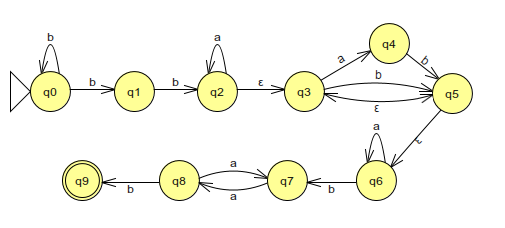
\includegraphics[width=11cm]{task3_NF}


	\item Детерминизировать один из построенных $\eps$-НКА. Верхние индексы для удобства.

	\begin{tabular}{lcccccccc}
		\toprule
		\multicolumn{1}{c}{
			$\delta^\prime \mid$
		}
		& \multicolumn{1}{c}{ $S^0$ }
		& \multicolumn{1}{c}{ $S1^1$ }
		& \multicolumn{1}{c}{ $S12356^2$ }
		& \multicolumn{1}{c}{ $23456^3$ }
		& \multicolumn{1}{c}{ $S123567^4$ }
		& \multicolumn{1}{c}{ $3567^5$ }
		& \multicolumn{1}{c}{ $234568^6$ }
		& \multicolumn{1}{c}{ $468^7$ }

		\\
		\midrule

		$a$ $\mid$ &
		--- & --- & $23456^3$ & $23456^3$ & $234568^6$ & $468^7$ & $234567^8$ &  $67^{10}$  \\
		$b$ $\mid$ &
		$S1^1$ & $S12356^2$ & $S123567^4$ & $3567^5$ & $S123567^4$ & $3567^5$ & $35679^9$ & $35679^9$ \\
		\bottomrule
	\end{tabular}

	\vspace{1em}

	\begin{tabular}{lccccc}
		\toprule
		\multicolumn{1}{c}{
			$\delta^\prime \mid$
		}
		& \multicolumn{1}{c}{ $35679^8$ }
		& \multicolumn{1}{c}{ $68^9$ }
		& \multicolumn{1}{c}{ $79^{10}$ }
		& \multicolumn{1}{c}{ $8^{11}$ }
		& \multicolumn{1}{c}{ $9^{12}$ }

		\\
		\midrule

		$a$ $\mid$ &
		$68^{11}$ & $67^{10}$ & $8^{14}$ & $8^{14}$ & --- & ---   \\
		$b$ $\mid$ &
		& $7^{12}$ & $79^{13}$ & --- & --- & $9^{15}$ & --- \\
		\bottomrule
	\end{tabular}

\end{enumerate}

\section*{Задание 1}

\begin{enumerate}[label=(\roman{*})]
	\setcounter{enumi}{5}
	\item Доказать, что $L(M^{ND}) = L(M^D) = L$.

	Так как мы получили $M^D$ путём детерминизации $M^{ND}$, то по теореме о редукции
	языки этих автоматов эквивалентны. Построение $M^{ND}$ производилось по регулярной грамматике, и по теореме Клини следует, что $L(G) = L(M^{ND})$. Равенство же $L(G) = L$ было доказано во втором пункте первого задания. Таким образом тождество доказано.

	Фактическое совпадение языков можно продемонстрировать следующим способом: в пункте (iii) мы вывели регулярное выражение для грамматики, а в пункте (viii) методом исключения получили регулярное выражение, описывающее язык автомата. Так как выражения совпадают, языки эквивалентны.

	\item Мимимизировать полученный конечный автомат, распознающий язык $L$, или доказать его минимальность.

	Рассмотрим $M^D$. Конечные состояния $CF$ и $CE$ являются эквивалентными, поэтому их можно совместить. Все остальные состояния различимы.

	 Отобразим этот автомат на диаграмме. (101 --- два состояния с тремя дугами.)

	 \begin{tikzpicture}[auto,>=stealth', node distance=3cm,auto,every state/.style={thick}]
	 \node (init) {};
	 \node[state] (qS) [right=.7cm of init] {$S$};
	 \node[state] (qA) [right of=qS] {$A$};
	 \node[state] (qB) [right of=qA] {$B$};
	 \node[state,accepting] (qCF) [right of=qB] {$CF$};
	 \node[state] (qKE) [right of=qCF] {$KE$};

	 \path[->]
	 (init) edge (qS)
	 (qS) edge [loop above] node {$0$} (qS)
	 (qS) edge node {$1$} (qA)
	 (qA) edge [loop above] node {$0$} (qA)
	 (qA) edge node {$1$} (qB)
	 (qB) edge [loop above] node {$0$} (qB)
	 (qB) edge node {$1$} (qCF)
	 (qCF) edge [bend left] node {$0$} (qKE)

	 (qKE) edge  [bend left] node {$101$} (qCF)
	 ;
	 \end{tikzpicture}

	\newpage
	\item Методом последовательного исключения состояний выписать регулярные
	выражения для $L(M^{ND})$, $L(M^D)$.\\

	$M^D$: Петли с нулём заменим на $0^*$, а цикл $CF-KE$ на $(1010)^*$, $L(M^D) = 0^*1\ 0^*1\ 0^*1\ (0101)^*$;


	\begin{tikzpicture}[auto,>=stealth', node distance=3cm,auto,every state/.style={thick}]
	\node (init) {};
	\node[state] (qS) [right=.7cm of init] {$S$};
	\node[state,accepting] (qCF) [right=2.5cm of qS] {$CF$};

	\path[->]
	(init) edge (qS)
	(qS) edge node {$0^*1\ 0^*1\ 0^*1$} (qCF)

	(qCF) edge [loop right] node {$0101$} (qCF)
	;
	\end{tikzpicture}

	$M^{ND}$: Стянем вершину $C$, после чего разобьём $SB$ на два пути: $SE, SF$.\\
	$L(M^{ND}) = (0^*1\ 0^*1\ 0^*1) + (0^*1\ 0^*1\ 0^*1\ (0101)^+) = 0^*1\ 0^*1\ 0^*1\ (0101)^*$.


	\begin{tikzpicture}[auto,>=stealth', node distance=3cm,auto,every state/.style={thick}]
	\node (init) {};
	\node[state] (qS) [right=.7cm of init] {$S$};
	\node[state] (qB) [right=2.5cm of qS] {$B$};
	\node[state,accepting] (qF) [right of=qB, below=0cm of qB] {$F$};
	\node[state,accepting] (qE) [right of=qB, above=0.1cm of qB] {$E$};

	\path[->]
	(init) edge (qS)
	(qS) edge node {$0^*1\ 0^*1\ 0^*$} (qB)
	(qB) edge node [above,rotate=-23] {$1$} (qF)
	(qB) edge node [above,rotate=23] {$1\ (0101)^+$} (qE)
	;
	\end{tikzpicture}

	\item Построить ДКА, распознающий дополнение $!L$ к языку $L$,
	записать $!L$ в виде регулярного выражения.

	Доопределим автомат до полного, преобразуем его в дополнение.

	\begin{tikzpicture}[auto,>=stealth', node distance=2cm,auto,every state/.style={thick}]
	\node (init) {};
	\node[state,accepting] (qS) [right=.7cm of init] {$S$};
	\node[state,accepting] (qA) [right of=qS] {$A$};
	\node[state,accepting] (qB) [right of=qA] {$B$};
	\node[state] (qCF) [right of=qB] {$CF$};
	\node[state,accepting] (qKE) [right of=qCF] {$KE$};
	\node[state,accepting] (qKU) [right of=qKE] {$KU$};
	\node[state,accepting] (qKL) [right of=qKU] {$KL$};
	\node[state,accepting] (C) [below of=qCF] {$C$};

	\path[->]
	(init) edge (qS)
	(qS) edge [loop above] node {$0$} (qS)
	(qS) edge node {$1$} (qA)
	(qA) edge [loop above] node {$0$} (qA)
	(qA) edge node {$1$} (qB)
	(qB) edge [loop above] node {$0$} (qB)
	(qB) edge node {$1$} (qCF)
	(qCF) edge node {$0$} (qKE)
	(qKE) edge node {$1$} (qKU)
	(qKU) edge node {$0$} (qKL)
	(qKL) edge [bend right] node [above] {$1$} (qCF)

	(qCF) edge node {$1$} (C)
	(qKE) edge [bend left] node [above] {$0$} (C)
	(qKU) edge [bend left] node [above] {$1$} (C)
	(qKL) edge [bend left] node [above] {$0$} (C)
	(C) edge [loop left] node {$0, 1$} (C)
	;
	\end{tikzpicture}

	Построим грамматику, порождающую этот автомат.
	\begin{equation}
		\begin{array}{l}
		S \to \eps \mid 0S \mid 1A, \\
		A \to \eps \mid 0A \mid 1B, \\
		B \to \eps \mid 0B \mid 1CF, \\
		CF \to 0KE \mid 1C, \\
		KE \to \eps \mid 1KU \mid 0C, \\
		KU \to \eps \mid 0KL \mid 1C, \\
		KL \to \eps \mid 1CF \mid 0C, \\
		C \to \eps \mid 1C \mid 0C;
		\end{array}
	\end{equation}

	Решим систему уравнений:\\

	$KE = 101CF + 1 + 10 + (0 + 11 + 100)(0+1)^* + \eps$,

	$CF = 0101CF + 0 + 01 + 010 + (1 + 00 + 011 + 0100)(0+1)^* + \eps$,

	$CF = (0101)^*(0 + 01 + 010 + (1 + 00 + 011 + 0100)(0+1)^* + \eps)$,

	$S = 0^*(\eps + 10^*(\eps + 10^*(\eps + 1CF))) = 0^* + 0^*10^* + 0^*10^*1\,CF$

	Ответ: $0^* + 0^*10^* + 0^*10^*1\,(0101)^*(0 + 01 + 010 + (1 + 00 + 011 + 0100)(0+1)^* + \eps)$.

\end{enumerate}



\end{document}
